\documentclass[conference]{IEEEtran}
\IEEEoverridecommandlockouts
\usepackage{cite}
\usepackage{amsmath,amssymb,amsfonts}
\usepackage{graphicx}
\usepackage{booktabs}
\usepackage{multirow}
\usepackage{xcolor}
\usepackage[hidelinks]{hyperref}
\graphicspath{{../figures/}{figures/}}

\begin{document}

\title{Fed-MediShield: Behaviour-Probing Defence Against Backdoor Attacks in Federated Intrusion Detection for the Internet of Medical Things}

\author{\IEEEauthorblockN{Author One}
\IEEEauthorblockA{\textit{Department} \\
\textit{Institution}\\
City, Country \\
email}
\and
\IEEEauthorblockN{Author Two}
\IEEEauthorblockA{\textit{Department} \\
\textit{Institution}\\
City, Country \\
email}
}

\maketitle

\begin{abstract}
Federated learning lets hospitals and device operators train a shared intrusion detection system (IDS) for the Internet of Medical Things (IoMT) without pooling sensitive traffic, but a few malicious participants can implant a backdoor that makes triggered attack traffic look benign. Geometry-based defences struggle here: a partially poisoned update looks like an honest update from a client with unusual data. We propose Fed-MediShield, a server-side defence that inspects what each update \emph{does} to the protected decision (``attack $\rightarrow$ benign'') rather than how it looks. The server probes every submitted model on a small trusted reference sample, scores how broadly the update shifts attack traffic towards the benign class relative to its peers and to the client's own known-clean profile, and converts the score into bounded aggregation weights, with retroactive revocation and a safe hold rule. In pre-registered experiments on CICIoMT2024 with fresh seeds, Fed-MediShield reduced the final attack success rate from 98.96\% to 0.29\% while keeping macro-F1 equal to undefended FedAvg; on the untouched official test split the attack success rate was 0.03\% versus 99.58\%. Compared with FedAvg and five robust baselines, it was the only method that removed the backdoor without utility loss, and the same pattern held on ToN-IoT. We report the limitations we observed: slower detection on ToN-IoT and with 32 clients, failure under extreme heterogeneity, and partial evasion by source-specific backdoors.
\end{abstract}

\begin{IEEEkeywords}
federated learning, backdoor attack, intrusion detection, Internet of Medical Things, robust aggregation
\end{IEEEkeywords}

\section{Introduction}
IoMT devices such as infusion pumps, monitors and wearables expand the attack surface of hospital networks, and recent surveys identify adversarially robust and privacy-preserving IDSs as an open need~\cite{hassan2025survey}. Federated learning (FL)~\cite{mcmahan2017fedavg} lets several sites train one IDS without exchanging raw traffic, but it is vulnerable to poisoning: a participant can train on traffic carrying a trigger relabelled as benign, so that the global model lets triggered attacks through while behaving normally otherwise~\cite{bagdasaryan2020backdoor}. For an IDS, this targeted evasion is the most damaging outcome.

Robust aggregation rules such as Krum~\cite{blanchard2017krum}, the coordinate-wise median and trimmed mean~\cite{yin2018median} and the geometric median (RFA)~\cite{pillutla2022rfa}, and detectors based on update distances or clustering~\cite{pathak2026early,bi2026hflmnd,zhang2022fldetector}, treat poisoned updates as geometric outliers. A backdoor client that poisons only part of its data, however, submits an update that is close to honest updates, while honest clients with skewed (non-IID) traffic can be far from the crowd. In our experiments, median, trimmed mean, RFA and the Hausdorff-distance detector Fed-ADH~\cite{pathak2026early} let the backdoor through ($\geq$97\% attack success), and Krum blocked it only by discarding most honest updates (macro-F1 $-$10 points).

Fed-MediShield instead asks what each update does to the decision we want to protect. Its contributions are:
\begin{itemize}
\item a behaviour-probing score that measures how broadly an update shifts attack traffic towards the benign class, relative to peers and to the client's own known-clean profile, so that honest non-IID clients are not penalised;
\item a bounded-influence aggregation with first-episode revocation and a hold rule, with $0 \le a_i \le p_i$ for every client;
\item a pre-registered evaluation on CICIoMT2024~\cite{dadkhah2024ciciomt} (including its official test split) and ToN-IoT~\cite{moustafa2021ton}, against five baselines, sweeps and adaptive attacks, with failures reported.
\end{itemize}

\section{Related Work}
\textbf{Backdoors in FL.} Bagdasaryan et al.~\cite{bagdasaryan2020backdoor} showed that a single participant can implant a backdoor; norm clipping limits but does not remove it~\cite{sun2019canyou}. DualVeil~\cite{zhang2026dualveil} makes backdoors persistent and inconspicuous, which motivates our persistence experiment.

\textbf{Robust aggregation and detection.} Krum~\cite{blanchard2017krum}, median and trimmed mean~\cite{yin2018median} and RFA~\cite{pillutla2022rfa} bound the influence of outlying updates. FLTrust~\cite{cao2021fltrust} scores clients against a server root dataset, FoolsGold~\cite{fung2020foolsgold} down-weights similar Sybils, and FLDetector~\cite{zhang2022fldetector} checks update consistency over time. In healthcare FL, Pathak et al.~\cite{pathak2026early} detect untargeted poisoning early with Hausdorff distances (Fed-ADH), and HFLMND~\cite{bi2026hflmnd} clusters similarity features with a historical suspicion score. These methods inspect update geometry; Fed-MediShield inspects the protected behaviour, using a trusted reference sample in the spirit of FLTrust's root data.

\section{Threat Model and Problem}
$N$ clients hold private traffic and train a $K$-class IDS by FedAvg-style rounds; client $i$ has nominal weight $p_i$ (its data share). A minority of clients is malicious (honest majority, as assumed in~\cite{bi2026hflmnd}). An attacker relabels a fraction of its attack rows to the benign class after applying a trigger $T$ to a few feature columns, trains normally otherwise, and participates every round unless stated otherwise. The attack success rate (ASR) is the share of triggered non-benign validation records classified as benign. The server sees model updates in plaintext, holds a small trusted reference sample (32 distinct records per class, removed from clients), and has known-clean training trajectories (e.g.\ from a vetted pilot phase) for calibration. It never sees attacker identities, trigger, poison masks or test data. The goal is to drive ASR to the undefended clean level while keeping accuracy, macro-F1 and rare-class recall equal to FedAvg.

\section{Fed-MediShield}

\begin{figure*}[t]
\centering
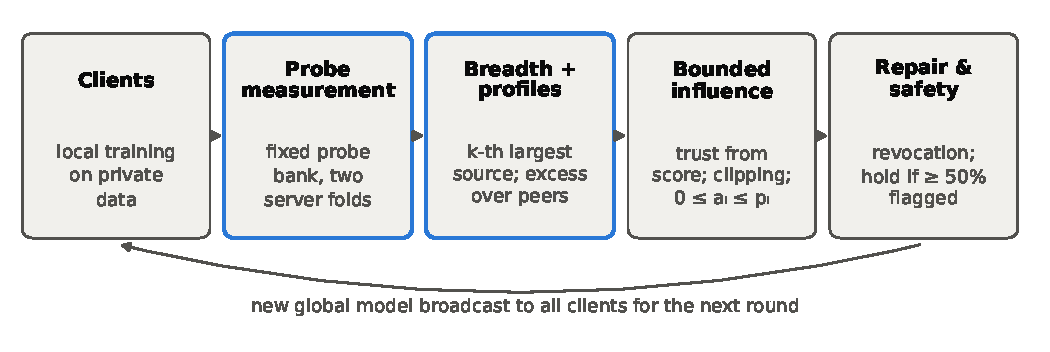
\includegraphics[width=0.92\textwidth]{fig0_method_overview}
\caption{Server pipeline of Fed-MediShield in each round.}
\label{fig:overview}
\end{figure*}

Fig.~\ref{fig:overview} summarises one round.

\textbf{Probe measurement.} The reference sample is split into two folds. A fixed bank $\mathcal{Q}$ of 588 probes perturbs groups of standardised features (contiguous groups of width 1, 2 and 4 plus 16 random groups, at levels $\pm3$ and $\pm6$). For client model $w_i$, global model $w$, probe $q$, true source class $s \neq b$ and output class $c$,
\begin{equation}
E_i[q,s,c] = \Delta_{w_i}[q,s,c] - \Delta_{w}[q,s,c],
\end{equation}
where $\Delta_w[q,s,c]$ is the mean change of $P_w(c \mid q(x)) - P_w(c \mid x)$ over reference records of class $s$. A trigger-based backdoor raises $E_i[q,s,b]$ for the benign class $b$ on probes that overlap the trigger.

\textbf{Breadth and specificity.} A trigger is input-agnostic, so it pushes many source classes towards $b$, whereas a legitimate local rule usually concerns one class. For each probe, the breadth statistic is the $k$-th largest value of $E_i[q,s,b]$ over source classes ($k=3$), minus the client's median over probes (specificity), which removes uniform shifts.

\textbf{Peer comparison and client profiles.} Each client's statistic is compared with the leave-one-out median and MAD of its peers; a probe is selected on the first fold and confirmed on the second, which suppresses chance maxima over the 588 probes. Clients with genuinely unusual data would still stand out, so we count only the excess above the larger of the peer median and the client's own profile, i.e.\ the 0.90 quantile of its score on known-clean calibration trajectories. This removed the honest false alarms that otherwise locked out a client whose legitimate rule the global model never absorbed.

\textbf{Calibration.} Alert thresholds are the 0.99 quantile plus a margin of the scores of known-clean trajectories, per training phase (rounds 1--3 and later), with a floor of 3. Calibration is validated by leave-one-seed-out transfer and by a live development gate on development seeds before any evaluation run.

\textbf{Bounded influence.} A score above the threshold raises a client risk $r_i$; its aggregation coefficient is
\begin{equation}
a_i = p_i\, e^{-r_i} \min\!\left(1, \frac{C}{\lVert \delta_i \rVert}\right), \qquad 0 \le a_i \le p_i,
\end{equation}
with clip bound $C$ from clean update norms. The new model is $w + \sum_i a_i \delta_i$; the unassigned mass $1 - \sum_i a_i$ stays on the previous model, so there is no renormalisation that would amplify the remaining updates.

\textbf{Revocation and hold rule.} The first poisoned round cannot be detected, so at a client's first detection episode the server subtracts its recent applied contributions (window of three rounds, at most $p_i$ per round). Later alerts attenuate the current update but do not revoke past honest work, which prevents oscillation under intermittent attacks. If half the clients are flagged or too little informative mass remains, the round is held (the global model is unchanged); three consecutive invalid rounds stop training.

\textbf{Properties.} (i) Influence is bounded: for the attacker set $\mathcal{A}$, $\lVert \sum_{i \in \mathcal{A}} a_i \delta_i \rVert \le C \sum_{i \in \mathcal{A}} p_i e^{-r_i}$, which vanishes as attacker risks grow. (ii) A held round cannot introduce poison, since nothing is applied. (iii) Server cost is linear in the number of clients: one probe pass per submitted model.

\section{Experimental Setup}
\textbf{Data.} CICIoMT2024~\cite{dadkhah2024ciciomt}: six classes (Benign, DDoS, DoS, Recon, MQTT, Spoofing) from one training file each, 45 features, a grouped 80/20 split that keeps identical feature vectors on one side, and the untouched official test files. ToN-IoT network data~\cite{moustafa2021ton}: ten classes (normal and nine attacks), identifiers (IP addresses and ports) and free-text fields removed, exact duplicates removed (one 15,344-row identical group otherwise dominated validation), 51 features.

\textbf{FL setup.} Eight clients with Dirichlet ($\alpha=0.5$) label skew, an MLP ($d$--128--64--$K$), AdamW (learning rate $10^{-3}$), two local epochs, batch 2048, 15 rounds, logit-adjusted cross-entropy ($\tau=0.5$)~\cite{menon2021logit}, which raised MQTT and Spoofing recall of the clean IDS.

\textbf{Attack.} Two of eight clients (25\%) poison 50\% of their attack rows from round 1. Triggers were selected before any attacked run so that clean models do not already map them to benign ($\leq$10\% per class): columns 5--8 set to 5 (CICIoMT2024) and four non-adjacent columns set to 5 (ToN-IoT).

\textbf{Baselines and metrics.} FedAvg~\cite{mcmahan2017fedavg}, Krum and median/trimmed mean ($f=2$)~\cite{blanchard2017krum,yin2018median}, RFA~\cite{pillutla2022rfa} and Fed-ADH~\cite{pathak2026early}, plus an evaluator-only oracle that drops the true attackers (perfect detection). We report ASR, accuracy, macro-F1, per-class recall, and detection recall and honest false-alarm rate over client updates.

\textbf{Protocol.} Design decisions used development seeds only. Confirmatory claims use fresh seeds with criteria fixed in advance; when a confirmation was not met we report it as such.

\section{Results}

\subsection{Main result and comparison}
On five fresh CICIoMT2024 seeds (pre-registered), Fed-MediShield lowered the final ASR from 98.96$\pm$1.97\% (FedAvg) to 0.29$\pm$0.32\%, detected 95.3\% of poisoned updates, and raised false alarms on 0.17\% of honest updates in clean runs; clean-run macro-F1 differed from FedAvg by $+0.18\pm0.40$ points, and attacked-run F1 matched the oracle ($+0.82\pm1.99$). Table~\ref{tab:compare} compares all methods. Only Fed-MediShield removed the backdoor with no utility loss; Krum removed it by excluding most honest updates (87.5\% of honest updates unselected in clean runs). On ToN-IoT the ranking was the same, with clean-run F1 identical to FedAvg and no honest update flagged. Fig.~\ref{fig:summary} shows that its attacked-run utility equals the oracle on both datasets.

\begin{table*}[t]
\centering
\caption{Comparison under the same attack (mean $\pm$ SD over seeds). CICIoMT2024: four conclusive seeds of 63--67 (FedAvg learned the backdoor); ToN-IoT: seeds 93--97 (descriptive, see Sec.~\ref{sec:limits}). Recall: share of poisoned updates flagged (attacked runs); FPR: share of honest updates flagged in clean runs; only for methods that flag clients.}
\label{tab:compare}
\setlength{\tabcolsep}{4pt}
\begin{tabular}{lcccccccc}
\toprule
& \multicolumn{4}{c}{CICIoMT2024} & \multicolumn{4}{c}{ToN-IoT} \\
\cmidrule(lr){2-5}\cmidrule(lr){6-9}
Method & ASR (\%) & Clean F1 & Recall & FPR & ASR (\%) & Clean F1 & Recall & FPR \\
\midrule
FedAvg~\cite{mcmahan2017fedavg} & 99.81$\pm$0.06 & 73.98$\pm$0.13 & -- & -- & 98.58$\pm$2.09 & 66.91$\pm$2.03 & -- & -- \\
Krum~\cite{blanchard2017krum} & 0.21$\pm$0.19 & 64.16$\pm$4.25 & 100 & 87.5 & 20.10$\pm$44.66 & 59.24$\pm$3.23 & 89.3 & 87.5 \\
Median~\cite{yin2018median} & 98.22$\pm$1.75 & 71.00$\pm$2.31 & -- & -- & 99.94$\pm$0.02 & 67.32$\pm$1.94 & -- & -- \\
Trimmed mean~\cite{yin2018median} & 97.61$\pm$1.72 & 72.32$\pm$2.03 & -- & -- & 99.92$\pm$0.04 & 68.87$\pm$2.91 & -- & -- \\
RFA~\cite{pillutla2022rfa} & 99.81$\pm$0.06 & 73.80$\pm$0.34 & -- & -- & 98.91$\pm$1.42 & 65.70$\pm$1.20 & -- & -- \\
Fed-ADH~\cite{pathak2026early} & 99.81$\pm$0.06 & 73.88$\pm$0.38 & 11.7 & 12.5 & 98.46$\pm$2.12 & 66.74$\pm$2.80 & 11.3 & 12.5 \\
\textbf{Fed-MediShield} & \textbf{0.05$\pm$0.03} & \textbf{73.98$\pm$0.13} & 95.0 & \textbf{0.0} & \textbf{0.12$\pm$0.08} & \textbf{66.91$\pm$2.03} & 81.3 & \textbf{0.0} \\
\bottomrule
\end{tabular}
\end{table*}

\begin{figure}[t]
\centering
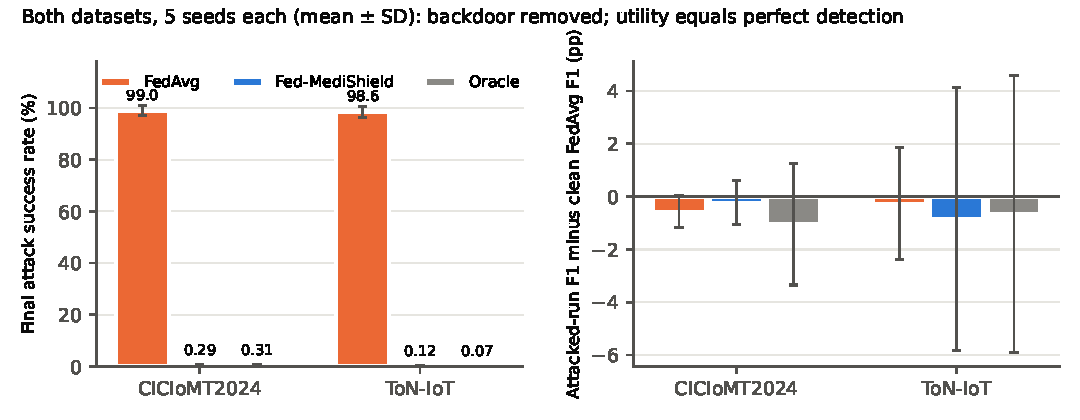
\includegraphics[width=\columnwidth]{fig11_two_dataset_summary}
\caption{Five seeds per dataset: final ASR (left) and attacked-run macro-F1 relative to clean FedAvg (right). Oracle: true attackers removed.}
\label{fig:summary}
\end{figure}

\subsection{Official test split}
The frozen final models were evaluated once on the official CICIoMT2024 test files (pre-registered). ASR was 0.03$\pm$0.04\% with Fed-MediShield and 99.58$\pm$0.57\% with FedAvg, and both reached the same accuracy (65.3\%) and flagged 99.1\% of attack traffic as malicious. Accuracy is lower than on validation (85\%) for every method because 98\% of the official DoS test flows are labelled DDoS: both classes are ICMP floods, indistinguishable per flow in the six-file subset. With the two flood classes merged (a supplementary, post-hoc analysis) test accuracy is 98.2\% for both methods.

\subsection{Robustness}
Table~\ref{tab:robust} summarises robustness tests of the final configuration (two development seeds for the delayed attack, three to five seeds otherwise). The backdoor was removed for all trigger types, attack schedules, poison rates and one to three attackers. With four of eight attackers (no honest majority) the hold rule paused training and then stopped it, which is the intended safe behaviour. In the persistence test the attack stopped after round 7: FedAvg kept the backdoor at about 96\% for eight further honest rounds, whereas Fed-MediShield kept it near zero and restored the former attackers' weight to 97\% once they behaved honestly. Fig.~\ref{fig:heat} shows where alerts are raised.

\begin{table}[t]
\centering
\caption{Robustness (final ASR, mean over seeds; FedAvg in brackets).}
\label{tab:robust}
\setlength{\tabcolsep}{3pt}
\begin{tabular}{lcc}
\toprule
Setting & Fed-MediShield & (FedAvg) \\
\midrule
Blended trigger (3 seeds) & 0.75--1.79\% & (82--96\%) \\
Trigger outside the probe bank & $\leq$0.64\% & (98--99\%) \\
Intermittent attacker & $\leq$0.71\% & (95--100\%) \\
Delayed attack (from round 8) & 0.02--0.03\% & (99.7--99.8\%) \\
1 / 2 / 3 attackers (5 seeds) & 0.04 / 0.05 / 0.17\% & (79 / 99 / 99.9\%) \\
Poison rate 0.2 / 0.35 / 0.8 & 0.07 / 0.05 / 0.09\% & (98 / 98 / 93\%) \\
Persistence (round 15) & 0.03--0.05\% & (95--96\%) \\
16 / 32 clients & 0.01--0.05 / 0.01--0.07\% & (97--100 / 96\%) \\
Dirichlet $\alpha=1.0$ & 0.02--0.08\% & (99.8\%) \\
\bottomrule
\end{tabular}
\end{table}

\begin{figure}[t]
\centering
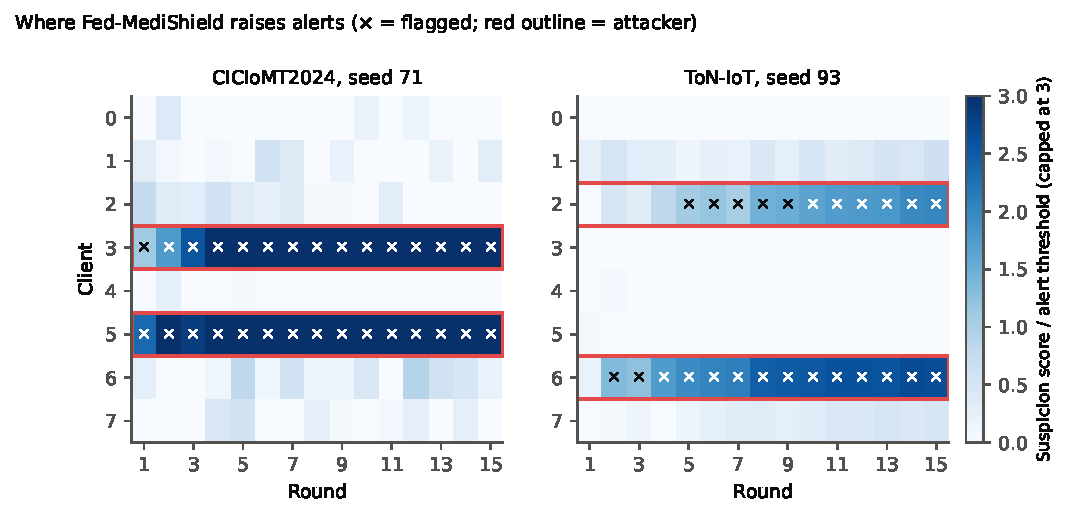
\includegraphics[width=\columnwidth]{fig10_detection_heatmaps}
\caption{Suspicion score relative to the alert threshold for each client and round (\texttimes: flagged; red frame: attacker).}
\label{fig:heat}
\end{figure}

\subsection{Ablation and cost}
Removing breadth ($k=1$) left the backdoor at 99.8\%; removing client profiles raised honest false alarms to 6.7\% and stopped one run; removing revocation let ASR reach 2--4\% during training. A history-based channel was removed during development because it produced 11 of 19 honest false alarms and no detection. Breadth is the one sensitive setting ($k=2$ or $4$ failed), whereas calibration quantile, margin, alert floor, profile quantile, revocation window and clip multiplier did not change the outcome. Server time was 0.68\,s per round for eight clients (0.65\,s probe measurement) with no client-side or communication overhead.

\section{Limitations}
\label{sec:limits}
(i) On ToN-IoT and with 32 clients, attackers with little data were often flagged only after more than three poisoned rounds (one client holding 0.3\% of the data never), so the backdoor was present in early rounds (mean ASR over rounds 8\% on ToN-IoT) before being removed; the pre-registered gate on detection timing was not met, and these results are therefore descriptive. (ii) Under extreme heterogeneity ($\alpha=0.1$) one attacker held 46\% of the data and could not be excluded without destroying utility. (iii) A source-specific backdoor that flips only one or two classes partly evades the breadth statistic (detection 31--77\%), although such backdoors were also weak without defence in our tests. (iv) Excluding attackers removes their genuine data; the oracle shows this cost is unavoidable. (v) The server needs plaintext updates and a trusted reference sample, which conflicts with secure aggregation. (vi) We used a six-file subset of CICIoMT2024, an MLP, synthetic feature-space triggers and up to 32 clients.

\section{Conclusion}
Fed-MediShield protects a federated IoMT IDS by probing the decision an attacker wants to change. Across pre-registered experiments it removed backdoors while keeping utility equal to FedAvg and to perfect detection, and it was the only method among FedAvg and five robust baselines to do both. Future work will address faster detection of small attackers, source-specific backdoors, adaptive attackers that optimise against the score, compatibility with secure aggregation, and the full CICIoMT2024 dataset.

\section*{Code Availability}
Code, protocols and result tables will be released at [repository and DOI to be added].

\bibliographystyle{IEEEtran}
\bibliography{references}

\end{document}
